% Intended LaTeX compiler: pdflatex
\documentclass[11pt]{article}
\usepackage[utf8]{inputenc}
\usepackage[T1]{fontenc}
\usepackage{graphicx}
\usepackage{longtable}
\usepackage{wrapfig}
\usepackage{rotating}
\usepackage[normalem]{ulem}
\usepackage{amsmath}
\usepackage{amssymb}
\usepackage{capt-of}
\usepackage{hyperref}
\author{Construção de compiladores I}
\date{}
\title{Apresentação da disciplina}
\hypersetup{
 pdfauthor={Construção de compiladores I},
 pdftitle={Apresentação da disciplina},
 pdfkeywords={},
 pdfsubject={},
 pdfcreator={Emacs 29.4 (Org mode 9.7.22)}, 
 pdflang={English}}
\begin{document}

\maketitle
\section*{Objetivos}
\label{sec:orgca11612}

\subsection*{Objetivos}
\label{sec:org56a0287}

\begin{itemize}
\item Apresentar a importância da construção de compiladores na formação de um cientista da computação.
\item Apresentar a ementa, critérios de avaliação e bibliografia da disciplina.
\end{itemize}
\subsection*{Objetivos}
\label{sec:org93e215a}

\begin{itemize}
\item Apresentar a visão geral de um compilador.
\end{itemize}
\section*{Compiladores}
\label{sec:org22f1067}

\subsection*{Como executamos programas?}
\label{sec:orgcd3cd06}
\begin{itemize}
\item Três técnicas principais
\begin{itemize}
\item Interpretação
\item Compilação
\item Virtualização.
\end{itemize}
\end{itemize}
\subsection*{Interpretação}
\label{sec:orga744a83}

\begin{itemize}
\item Código fonte é representado como uma estrutura de dados e
o intepretador executa o programa diretamente.
\item Interpretador é responsável pela execução do programa e de
sua interação com o S.O.
\end{itemize}
\subsection*{Compilação}
\label{sec:orgaf676e0}

\begin{itemize}
\item Código fonte é traduzido para uma nova linguagem.
\item Código alvo pode ser uma linguagem de alto nível (transpilação).
\item Código alvo pode ser uma linguagem de baixo nível (compilação).
\end{itemize}
\subsection*{Virtualização}
\label{sec:org19f7c23}

\begin{itemize}
\item Código fonte é traduzido para uma linguagem de baixo nível, não diretamente entendida
pelo hardware.
\item Normalmente, chamado de bytecode.
\item Intepretadores mais eficientes.
\end{itemize}
\section*{Visão geral (montanha)}
\label{sec:org12377e8}

\begin{center}
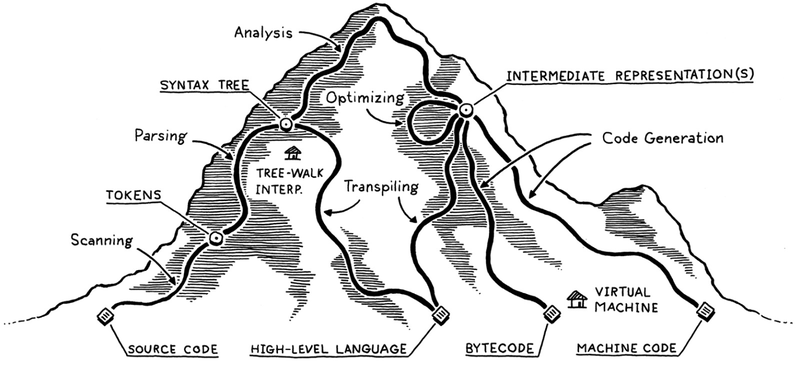
\includegraphics[width=.9\linewidth]{ montain.png}
\end{center}
\subsection*{Escalando a montanha}
\label{sec:org598c3ef}

\begin{itemize}
\item Análise Léxica: Dividir o código em \textbf{\textbf{tokens}}.
\begin{itemize}
\item Eliminar comentários e espaços em branco.
\end{itemize}
\end{itemize}
\subsection*{Escalando a montanha}
\label{sec:orge925c9c}

\begin{itemize}
\item Análise sintática: Organiza a sequência de tokens em sua estrutura gramatical.
\begin{itemize}
\item Produz uma árvore de sintaxe abstrata.
\end{itemize}
\end{itemize}
\subsection*{Escalando a montanha}
\label{sec:orgfcac9ba}

\begin{itemize}
\item Análise semântica: Verifica se a árvore produzida pelo analisador sintático atende restrições semânticas.
\begin{itemize}
\item Todos os símbolos foram declarados?
\item Argumentos de funções possuem a aridade e tipo corretos?
\end{itemize}
\end{itemize}
\subsection*{Escalando a montanha}
\label{sec:orgd43d5b9}

\begin{itemize}
\item Intepretador: executa o código diretamente a partir da árvore de sintaxe.
\begin{itemize}
\item Não há geração de código
\item Comum em linguagens dinamicamente tipadas, como Python.
\end{itemize}
\end{itemize}
\subsection*{Escalando a montanha}
\label{sec:org8de6e07}

\begin{itemize}
\item ``Transpilador'': converte a árvore de sintaxe para outra linguagem de alto nível.
\begin{itemize}
\item Ideal para permitir independência de plataformas.
\item Exemplo: Typescript.
\end{itemize}
\end{itemize}
\subsection*{Escalando a montanha}
\label{sec:org7504826}

\begin{itemize}
\item Geração de código intermediário: código de baixo nível independente de plataforma.
\begin{itemize}
\item Utilizado para otimizações independentes de hardware.
\end{itemize}
\end{itemize}
\subsection*{Escalando a montanha}
\label{sec:orgd6d2d96}

\begin{itemize}
\item Otimização de código.
\begin{itemize}
\item Otimização de consumo de memória, tempo de execução, tamanho de código, etc\ldots{}
\end{itemize}
\end{itemize}
\subsection*{Escalando a montanha}
\label{sec:org9f6661c}

\begin{itemize}
\item Geração de código: tradução da representação intermediária para o código de máquina,
diretamente executável pelo hardware.
\end{itemize}
\subsection*{Escalando a montanha}
\label{sec:orgbb55999}

\begin{itemize}
\item Virtualização: geração de código para máquinas virtuais como a JVM / EVM.
\begin{itemize}
\item Diferentes plataformas podem executar o mesmo programa utilizando VMs para a plataforma.
\end{itemize}
\end{itemize}
\section*{Motivação}
\label{sec:org62a6ed3}

\subsection*{Porque estudar compiladores?}
\label{sec:org9443c19}

\begin{itemize}
\item Desenvolver um compilador permite consolidar conhecimentos de:
\begin{itemize}
\item Teoria da computação (autômatos e gramáticas)
\end{itemize}
\end{itemize}
\subsection*{Porque estudar compiladores?}
\label{sec:org75daf60}

\begin{itemize}
\item Desenvolver um compilador permite consolidar conhecimentos de:
\begin{itemize}
\item Engenharia de software (testes e arquitetura de software)
\end{itemize}
\end{itemize}
\subsection*{Porque estudar compiladores?}
\label{sec:org52b31a7}

\begin{itemize}
\item Desenvolver um compilador permite consolidar conhecimentos de:
\begin{itemize}
\item Arquitetura de computadores (conhecer detalhes do alvo de compilação)
\end{itemize}
\end{itemize}
\subsection*{Porque estudar compiladores?}
\label{sec:orgd86e055}

\begin{itemize}
\item Possivelmente, o primeiro artefato de software complexo produzido por estudantes de graduação.
\end{itemize}
\subsection*{Porque estudar compiladores?}
\label{sec:orgb236f33}

\begin{itemize}
\item Compiladores aparecem em toda parte!
\begin{itemize}
\item Navegadores web (JavaScript e WebASM)
\end{itemize}
\end{itemize}
\subsection*{Porque estudar compiladores?}
\label{sec:org023ef13}

\begin{itemize}
\item Compiladores aparecem em toda parte!
\begin{itemize}
\item Monitoramento do Kernel Linux (eBPF)
\end{itemize}
\end{itemize}
\subsection*{Porque estudar compiladores?}
\label{sec:orgb51400d}

\begin{itemize}
\item Compiladores aparecem em toda parte!
\begin{itemize}
\item Várias aplicações possuem linguagens para customização.
\end{itemize}
\item Exemplos:
\begin{itemize}
\item VBA, elisp, Lua
\end{itemize}
\end{itemize}
\subsection*{Porque estudar compiladores?}
\label{sec:org4d329b7}

\begin{itemize}
\item Projeto de compiladores envolve problemas difíceis:
\begin{itemize}
\item Executam várias tarefas e devem ser eficientes.
\end{itemize}
\end{itemize}
\subsection*{Porque estudar compiladores?}
\label{sec:org83629e4}

\begin{itemize}
\item Projeto de compiladores envolve problemas difíceis:
\begin{itemize}
\item Responsáveis por bom uso de uma linguagem.
\end{itemize}
\end{itemize}
\subsection*{Porque estudar compiladores?}
\label{sec:orgce6ce50}

\begin{itemize}
\item Projeto de compiladores envolve problemas difíceis:
\begin{itemize}
\item Devem ocultar detalhes de arquitetura e SO de desenvolvedores.
\end{itemize}
\end{itemize}
\subsection*{Porque estudar compiladores?}
\label{sec:org9d94dd8}

\begin{itemize}
\item Provavelmente, uma das áreas mais consolidadas da ciência da computação!
\end{itemize}
\subsection*{Porque estudar compiladores?}
\label{sec:orgb002745}

\begin{itemize}
\item Vários pesquisadores da área foram agraciados com o Turing Award!
\begin{itemize}
\item John Backus, Barbara Liskov, Niklaus Wirth, Edsger Djikstra, Robin Milner e C.A. Hoare.
\end{itemize}
\end{itemize}
\subsection*{Porque estudar compiladores?}
\label{sec:orgb9c35c2}

\begin{itemize}
\item A área de linguagens de programação, apesar de teórica, possui demanda de vagas!
\begin{itemize}
\item Áreas de atuação: ferramentas de análise estática de código e teste automatizado.
\item Verificação formal de aplicações WEB3 (contratos inteligentes).
\item Segurança de software.
\end{itemize}
\end{itemize}
\subsection*{Porque estudar compiladores?}
\label{sec:org4ccf3cf}

\begin{itemize}
\item Como determinar se o bug em seu código está presente em seu programa fonte ou foi inserido durante o processo de compilador?
\end{itemize}
\subsection*{Porque estudar compiladores?}
\label{sec:org7b1d275}

\begin{itemize}
\item Correção de um compilador é um problema sério!

\item Como determinar se um compilador é ou não correto?
\begin{itemize}
\item Código produzido pelo compilador deve ter o mesmo significado que o código fonte original.
\end{itemize}
\end{itemize}
\subsection*{Porque estudar compiladores?}
\label{sec:org7c2d747}

\begin{itemize}
\item Qual o problema da compilação?

\item Imagine a situação:
\begin{itemize}
\item Dado um programa fonte P, o compilador produz o código alvo E, que é equivalente a P, exceto que E imprime um ``Hello world'' adicional.
\end{itemize}
\end{itemize}
\subsection*{Porque estudar compiladores?}
\label{sec:org259090c}

\begin{itemize}
\item Pode-se pensar, um print adicional é inócuo\ldots{}
\begin{itemize}
\item Depende da informação impressa!
\item Informações: endereços de memória restritos, versões de software instalado\ldots{}
\item Executar programas na máquina host durante a execução
\end{itemize}
\end{itemize}
\subsection*{Porque estudar compiladores?}
\label{sec:orgce5059e}

\begin{itemize}
\item Pesquisa em compiladores?
\begin{itemize}
\item Como produzir código mais eficiente? Otimização de código.
\item Como garantir que um compilador é correto? Verificação e teste.
\item Criar novas linguagens e seus compiladores.
\end{itemize}
\end{itemize}
\subsection*{Porque estudar compiladores?}
\label{sec:org100ee61}

\begin{itemize}
\item Pesquisa realizada no DECOM / UFOP
\begin{itemize}
\item Novos algoritmos para análise sintática / léxica.
\item Verificação e teste de programas.
\item Análise de código fonte.
\end{itemize}
\end{itemize}
\subsection*{Porque estudar compiladores?}
\label{sec:orgc9fd063}

\begin{itemize}
\item Novos algoritmos para análise sintática / léxica
\begin{itemize}
\item Terminação de análise sintática usando PEGs.
\item Análise léxica utilizando derivadas.
\item Análise sintática de formatos binários usando PEGs.
\end{itemize}
\end{itemize}
\subsection*{Porque estudar compiladores?}
\label{sec:orgf317dca}

\begin{itemize}
\item Verificação e teste de programas.
\begin{itemize}
\item Filtros de pacotes e extensões de Kernel (eBPF).
\begin{itemize}
\item Teste automatizado de programas.
\item Verificação formal baseada em assistente de provas.
\end{itemize}
\end{itemize}
\end{itemize}
\subsection*{Porque estudar compiladores?}
\label{sec:orge376a21}

\begin{itemize}
\item Verificação e teste programas.
\begin{itemize}
\item Análise de complexidade assintótica de tempo.
\end{itemize}
\item Análise de código fonte
\begin{itemize}
\item Desenvolvimento de bibliotecas para manipulação de código.
\end{itemize}
\end{itemize}
\section*{Estrutura de um compilador}
\label{sec:orgb31c56c}

\subsection*{Estrutura geral}
\label{sec:org47b0b08}

\begin{itemize}
\item Estrutura geral de um compilador
\end{itemize}

\begin{center}
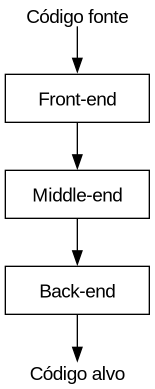
\includegraphics[width=.9\linewidth]{compiler_structure.png}
\label{}
\end{center}
\subsection*{Front-end de um compilador}
\label{sec:org1ccda29}

\begin{itemize}
\item Responsável pela análise do código.
\item Produz uma representação intermediária para geração de código.
\end{itemize}
\subsection*{Middle-end de um compilador}
\label{sec:org7787988}

\begin{itemize}
\item Responsável por otimizações independentes de arquitetura.
\begin{itemize}
\item Constant folding: substituir 3 + 4 por 7 no código.
\item Dead code elimination: eliminar código que nunca é executado.
\item Loop unrolling: eliminar laços para reduzir custo de desvios.
\end{itemize}
\end{itemize}
\subsection*{Back-end de um compilador}
\label{sec:orgff2f145}

\begin{itemize}
\item Responsável por otimizações dependentes do hardware.
\begin{itemize}
\item Alocação de registradores: como usar registradores da melhor maneira?
\item Escalonamento de instruções: qual a ordem de instruções para melhor eficiência?
\item Otimizações específicas de arquitetura: usar vectorização, múltiplos núcleos.
\end{itemize}
\end{itemize}
\subsection*{Porque essa arquitetura?}
\label{sec:org3f9c81a}

\begin{itemize}
\item Um mesmo front-end pode suportar diferentes middle-ends, sem modificações na linguagem fonte.
\item Um mesmo middle-end pode suportar diferentes arquiteturas.
\item Separação permite que desenvolvimento seja focado em problemas de cada componente.
\end{itemize}
\subsection*{Exemplos}
\label{sec:orgf6252e0}

\begin{center}
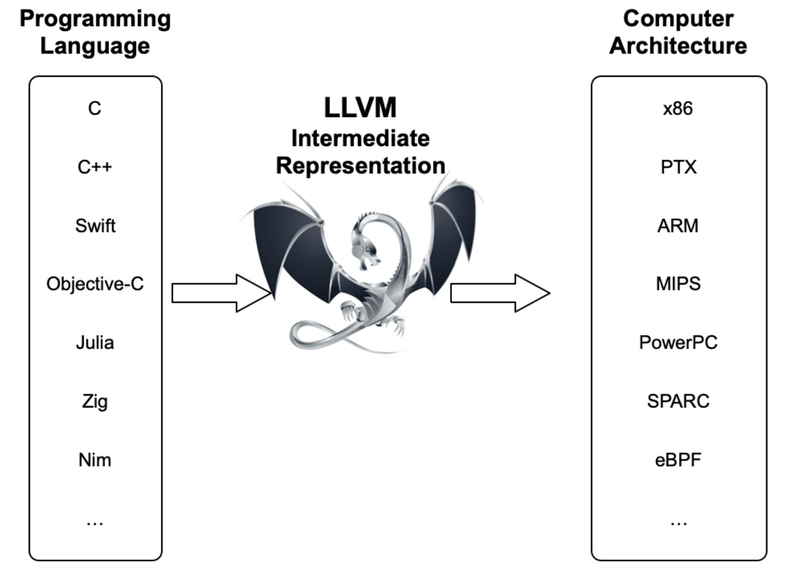
\includegraphics[width=.9\linewidth]{ llvm1.png}
\end{center}
\subsection*{Exemplos}
\label{sec:org34933fe}

\begin{center}
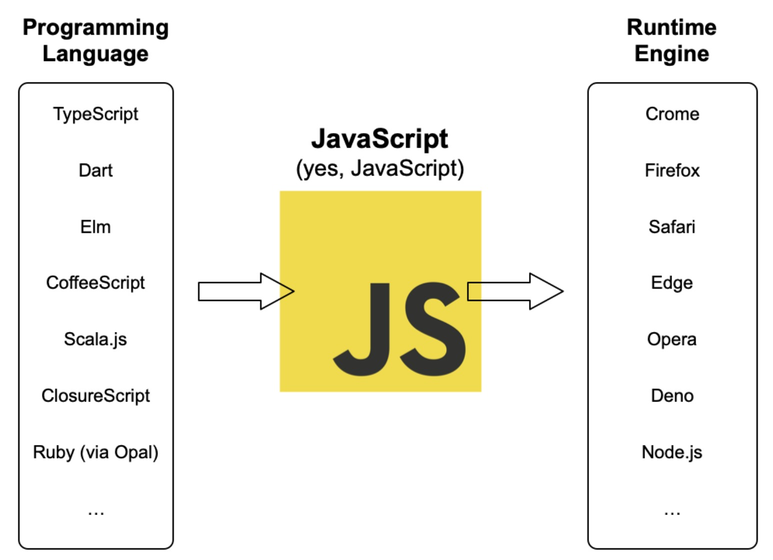
\includegraphics[width=.9\linewidth]{ javascript.png}
\end{center}
\subsection*{Exemplos}
\label{sec:org4d611ae}

\begin{center}
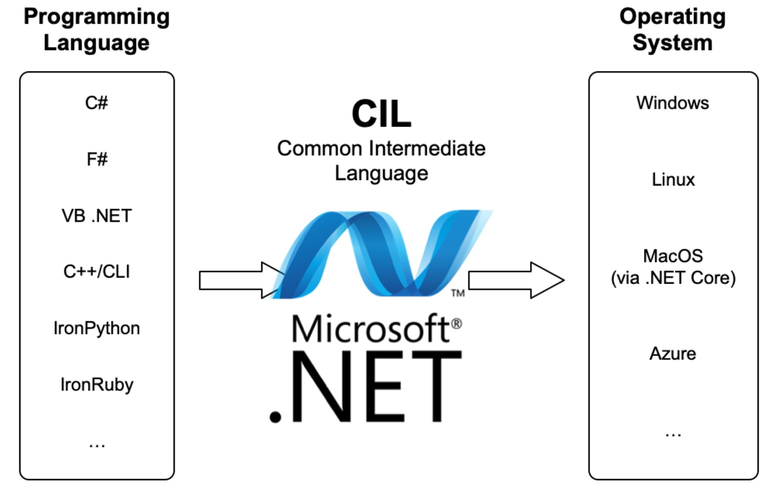
\includegraphics[width=.9\linewidth]{ net.png}
\end{center}
\subsection*{Exemplos}
\label{sec:org14fc241}

\begin{center}
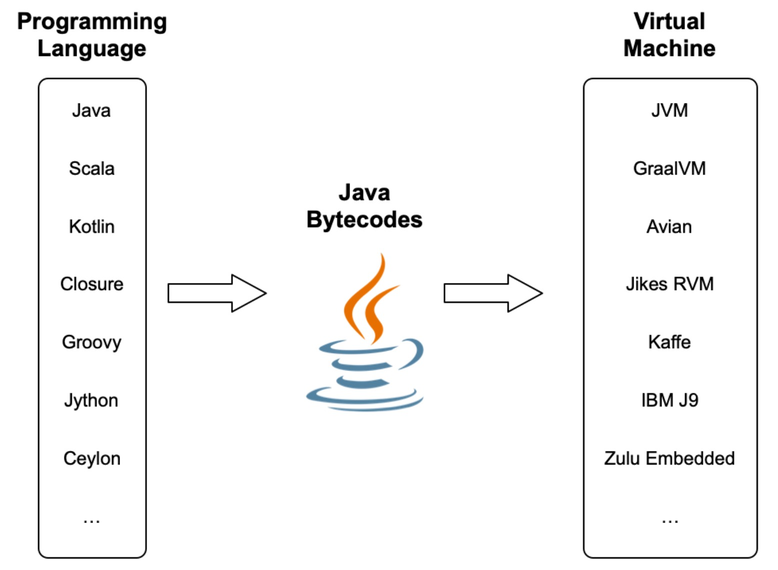
\includegraphics[width=.9\linewidth]{ java.png}
\end{center}
\section*{Ementa}
\label{sec:org3017216}

\subsection*{Ementa}
\label{sec:org62f3205}

\begin{itemize}
\item Introdução ao processo de compilação e interpretação

\item Análise léxica

\item Análise sintática

\item Análise semântica e geração de código intermediário.
\end{itemize}
\subsection*{Pré-requisitos}
\label{sec:org632eb8e}

\begin{itemize}
\item Essa disciplina faz uso \textbf{\textbf{INTENSO}} de conceitos:
\begin{itemize}
\item BCC222 Programação Funcional
\item BCC244 Teoria da Computação
\end{itemize}
\end{itemize}
\subsection*{Pré-requisitos}
\label{sec:org230940b}

\begin{itemize}
\item BCC222 Programação funcional
\begin{itemize}
\item Tipos de dados algébricos e casamento de padrão.
\item Polimorfismo paramétrico e sobrecarga.
\item Mônadas, functores e functores aplicativos.
\end{itemize}
\end{itemize}
\subsection*{Pré-requisitos}
\label{sec:orgf20f26d}

\begin{itemize}
\item BCC244 Teoria da computação
\begin{itemize}
\item Autômatos finitos determinísticos, não determinísticos e expressões regulares.
\item Gramáticas livres de contexto, ambiguidade e manipulação de gramáticas.
\end{itemize}
\end{itemize}
\section*{Bibliografia}
\label{sec:org506a1b6}

\subsection*{Bibliografia}
\label{sec:orgf5b6934}

\begin{itemize}
\item Construindo Compiladores. Cooper, Keith D. ; Torcson, Linda

\item Compiladores: Princípios, técnicas e ferramentas. Aho, Alfred; Lam,
Monica; Sethi, Ravi; Ullman, Jeffrey.

\item Modern compiler implementation in ML. Appel, Andrew.
\end{itemize}
\section*{Materiais de apoio}
\label{sec:orgee7c105}

\subsection*{Materiais de apoio}
\label{sec:orgdb40a5e}

\begin{itemize}
\item Slides e código de exemplo serão disponibilizados no seguinte
repositório online.
\end{itemize}
\section*{Critérios de Avaliação}
\label{sec:org11bdddc}

\subsection*{Critérios de Avaliação}
\label{sec:orgbb575e4}

\begin{itemize}
\item Duas avaliações no valor de 6,0 pontos.

\item Exercícios de programação no valor 4,0 pontos.
\end{itemize}
\subsection*{Critérios de Avaliação}
\label{sec:orge04f4aa}

\begin{itemize}
\item Exercícios de programação
\begin{itemize}
\item Desenvolvimento incremental de uma linguagem de programação simples
\end{itemize}
\item Implementação
\begin{itemize}
\item Compilação para uma máquina virtual.
\item Interpretador.
\end{itemize}
\end{itemize}
\subsection*{Critérios de Avaliação}
\label{sec:orgdd941cb}

\begin{itemize}
\item Datas de entregas de exercícios serão postadas na plataforma Moodle.
\begin{itemize}
\item Entrega via Github classroom.
\end{itemize}

\item Trabalhos serão individuais.
\end{itemize}
\subsection*{Critérios de Avaliação}
\label{sec:orgc6146c9}

\begin{itemize}
\item Data avaliação 1: 30/06/2025
\item Data avaliação 2: 25/08/2025
\end{itemize}
\subsection*{Exame especial}
\label{sec:orgcf8aabd}

\begin{itemize}
\item Mínimo de 75\% de frequência e nota inferior a 6,0.

\item Exame especial parcial para alunos que perderam uma avaliação.

\begin{itemize}
\item Envolverá tarefas de codificação e atividades teóricas (em papel).
\end{itemize}

\item Detalhes: Resolução CEPE 2880 de 05/2006
\end{itemize}
\subsection*{Exame especial}
\label{sec:orgbfbdb04}

\begin{itemize}
\item Data do exame especial: 01/09/2025
\end{itemize}
\section*{Software}
\label{sec:orge4f4a0c}

\subsection*{Software}
\label{sec:org7b9ce34}

\begin{itemize}
\item Trabalhos e códigos de exemplo serão desenvolvidos utilizando Haskell.

\item Utilizaremos diversas bibliotecas da linguagem Haskell.
\end{itemize}
\subsection*{Software}
\label{sec:org1bd78dc}

\begin{itemize}
\item Para evitar problemas de compatibilidade, será fornecido um ambiente de desenvolvimento baseado em Docker.

\item Trabalhos que apresentarem qualquer erro de compilação neste ambiente, não serão considerados para correção.
\end{itemize}
\section*{Outras Informações}
\label{sec:org867d311}

\subsection*{Informações}
\label{sec:orge9468cf}

\begin{itemize}
\item Toda informação da disciplina será disponibilizada na plataforma
Moodle.

\item Email: rodrigo.ribeiro@ufop.edu.br
\end{itemize}
\subsection*{Atendimento}
\label{sec:org973ceea}

\begin{itemize}
\item Horários de atendimento
\begin{itemize}
\item Segunda-feira: 17:00 - 19:00h
\item Terça-feira: 13:00 - 18:00h
\end{itemize}
\item Gentileza, agendar por e-mail atendimentos na segunda-feira.
\end{itemize}
\section*{Finalizando}
\label{sec:org1fa7453}

\begin{itemize}
\item Tenhamos todos um excelente semestre de trabalho!
\end{itemize}
\end{document}
